\documentclass[../Head/Main.tex]{subfiles}
\begin{document}
\begin{figure}[H]
	\centering
	\begin{subfigure}[b]{0.49\textwidth}
		\centering
		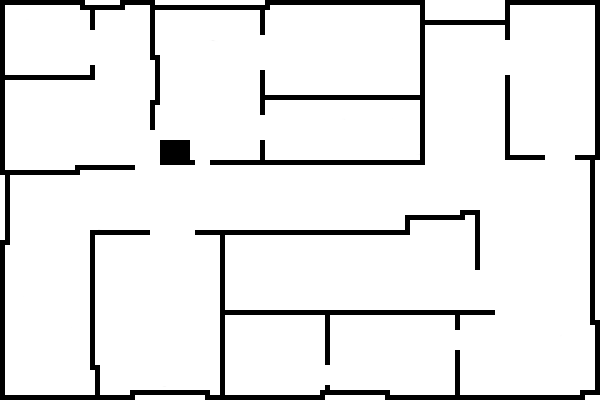
\includegraphics[width=\textwidth]{Maps/map_medium_white}
		\caption{Illustration of the world "bigworld"}
		\label{fig:bigworld_white}
	\end{subfigure}
	\hfill	
	\begin{subfigure}[b]{0.49\textwidth}
		\centering
		\begin{tikzpicture}
		\node[anchor=south west, inner sep=0] (image) at (0,0) {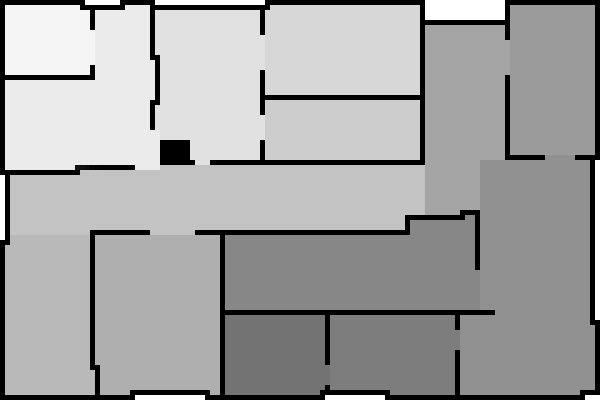
\includegraphics[width=\textwidth]{Maps/map_medium}};
		\node[align=center, black, font={\small}] at (0.7,5) {Room 1};
		\node[align=center, black, font={\small}] at (1.2,3.9) {Room 2};
		\node[align=center, black, font={\small}] at (2.9,4.5) {Room 3};
		\node[align=center, black, font={\small}] at (4.75,4.9) {Room 4};
		\node[align=center, black, font={\small}] at (4.76,3.75) {Room 5};
		\node[align=center, black, font={\small}] at (3,2.75) {Room 6};
		\node[align=center, black, font={\small}] at (0.65,1.25) {Room 7};
		\node[align=center, black, font={\small}] at (2.2,1.25) {Room 8};
		\node[align=center, black, font={\small}] at (6.45,4.25) {Room 9};
		\node[align=center, black, font={\small}] at (7.7,4.5) {Room 10};
		\node[align=center, black, font={\small}] at (7.5,1.75) {Room 11};
		\node[align=center, black, font={\small}] at (4.75,1.8) {Room 12};
		\node[align=center, black, font={\small}] at (5.45,0.6) {Room 13};
		\node[align=center, black, font={\small}] at (3.8,0.6) {Room 14};
		\end{tikzpicture}		
		\caption{"bigworld" divided into 14 rooms}
		\label{fig:bigworld_14_rooms}
	\end{subfigure}
	\caption{Illustration of the world "bigworld" before and after it has been divided into 14 rooms}
	\label{fig:bigworld}
\end{figure}
\end{document}